
\section{Neural Networks}
\label{sec:neural_networks}
	
	In this section we will see how neural network manage to solve classification tasks. As a reminder, a classification problem aims at identifying the sub-populations of a set belonging to a class. More specifically : we are given a set of inputs $X$ and outputs $Y$ composed by $n$ samples. We denote $x_i$ a sample of the set $X$. This sample $x_i$ is belongs to the class $y_i$. The aim of classification is, given a new sample $x_i$ to find the best matching class $y_i$ it belongs in.

	The algorithms we use in this report are the artificial neural networks. they are a family of statistical learning algorithms. They are inspired from the human brain structure : nowadays, we believe the brain has a network of neurons triggering signals over its dendrite and propagated to other neurons through a synapse interface. Network of artificial neurons mimics these properties.

	\vspace{1em}
	\textbf{Notation : }\\
	We mentioned that the input set $X$ and output set $Y$ were composed by $n$ samples where $x_i$ and $y_i$ denoted the specific input and true class output of the sample $i$. 
	\begin{itemize}
		\item $x_i$, the input vector of sample $i$, is a vector of size $m_1$, which means that the input $x_i$ is represented by $m_1$ different features, we note $x_{ij}$ the value of feature $j$ of sample $i$.
		\item $y_i$, the true class output of sample $i$, is a vector of size $m_2$, which means that the samples in $X$ can belong in $m_2$ different classes. We denote $y_{ij}$ the value of the output for the class $j$ of sample $i$.
		\item $p_i$, the prediction output of sample $i$, is a vector of size $m_2$. It represents the prediction made by the model as it was feed with $x_i$. It tries to predict $y_i$. We denote $p_{ij}$ the value of the prediction for class $j$ of sample $i$.
	\end{itemize} 


	\subsection{Artificial neuron and Perceptron}
		Perceptrons, introduced by Rosenblatt in 1958 \cite{rosenblatt1958perceptron}, was the first artificial neuron introduced in the literature. \Fref{fig:perceptron} is a model of an artificial neuron. On this model, the $x_{ij}$s represent binary inputs of the perceptron and the perceptron, represented with a circle on the figure, is defined by a threshold activation function such that :

		$$ f(x_i) = \begin{cases}1 & \text{if } \sum_j \beta_j \cdot x_{ij} + b > 0\\0 & \text{otherwise}\end{cases}  $$ 

		Where $\beta_j$ is a weight assigned to the $x_{ij}$ input and $b$ is a bias terms that does not depend on any input value.

		We often consider a vector representation of the inputs such that $x_i$ is the vector composed by all the $x_{ij}$ and $\beta$ the vector composed by the $\beta_j$. In this case, we rewrite : 

		$$ f(x_i) = \begin{cases}1 & \text{if } \beta \cdot x_i + b > 0\\0 & \text{otherwise}\end{cases}  $$ 

		\begin{figure}
			\centering
			\def\layersep{1.5cm}
			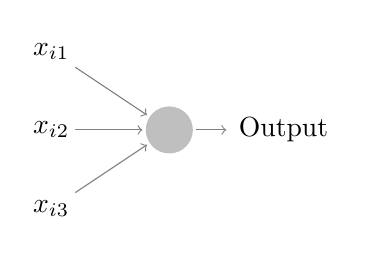
\begin{tikzpicture}[shorten >=1pt,->,draw=black!50, node distance=\layersep]
				\tikzstyle{tata}=[,minimum size=17pt,inner sep=0pt]
			    \tikzstyle{neuron}=[circle,fill=black!25,minimum size=17pt,inner sep=0pt]
			    \tikzstyle{output neuron}=[neuron, fill=red!50];

			    % Input neurons
			    \node[tata] (x1) at (\layersep,-1 cm) {$x_{i1}$};
			    \node[tata] (x2) at (\layersep,-2 cm) {$x_{i2}$};
			    \node[tata] (x3) at (\layersep,-3 cm) {$x_{i3}$};
			    
			    % Draw the output layer node
			    \node[neuron,pin={[pin edge={->}]right:Output}, right of=x2] (O) {};

			    % Connect every node in the hidden layer with the output layer
			    \path (x1) edge (O);
			    \path (x2) edge (O);
			    \path (x3) edge (O);

			\end{tikzpicture}
			\label{fig:perceptron}
			\caption{Model of an artificial neuron}
		\end{figure}

		The modern artificial neurons, like the sigmoid neuron, have the same representation as the model visible on \fref{fig:perceptron}. The differences comes from the inputs $x_i$ which are now real valued and the activation function that outputs a real value too. For instance, the sigmoid activation function is defined as : 

		$$ f(x_i) = \frac{1}{1+e^{-(\beta \cdot x_i + b)}} = \sigma(\beta \cdot x_i + b)  $$

		Where $\sigma(x_i)$ is the sigmoid function : $\sigma(x) = \frac{1}{1+e^{-x_i}}$



	\subsection{Neural network}
		Now that we have neurons, we need a network of them to compose an architecture similar to the brain one. The networks we are going to work with are feed-forward neural networks. They are the most common ones in the literature. \Fref{fig:feed_forward} is a representation of a two-hidden-layer feed-forward neural network. As you can see, that model consist of groups of neurons. We denote as layer the group of neurons belonging to the same deepness in the model. Therefore, all the neurons visible on the left in our model, compose the first layer of neurons. It's the input layer. The following layers are called the hidden layers and the last one is the output layer. Some variations exists of this definition, for instance, some outputs of the model might be placed at the level of a hidden layer.

		Consider our feed-forward model on \fref{fig:feed_forward}. If you feed this model with an input vector $x_i$ (composed by 4 features) then, going through the weights and neurons, the model will output a prediction $p_i$. This $p_i$ correspond to which classes the model believes $x_i$ belongs.
		

		\begin{figure}
			\centering
			\def\layersep{1.5cm}
			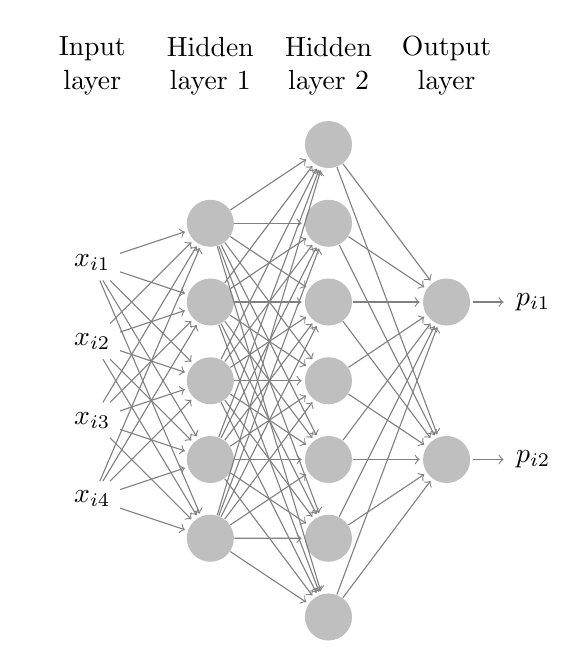
\begin{tikzpicture}[shorten >=1pt,->,draw=black!50, node distance=\layersep]
			    \tikzstyle{every pin edge}=[<-,shorten <=1pt]
			    \tikzstyle{neuron}=[circle,fill=black!25,minimum size=17pt,inner sep=0pt]
			    \tikzstyle{annot} = [text width=4em, text centered]


			    %%%%%%%%%%%%%%%%%%%%%%%%%%%%%%%%%%%%%%%%%%%% 
			    %%% DRAW THE NODES
			    %%%%%%%%%%%%%%%%%%%%%%%%%%%%%%%%%%%%%%%%%%%%
			    \foreach \name / \y in {1,...,4}
			        \node[] (I-\name) at (0,-\y) {$x_{i\y}$};

			    \foreach \name / \y in {1,...,5}
			        \path[yshift=0.5cm] node[neuron] (H1-\name) at (\layersep,-\y cm) {};

				\foreach \name / \y in {1,...,7}
			        \path[yshift=1.5cm] node[neuron] (H2-\name) at (\layersep*2,-\y cm) {};   

		       	
			    \node[neuron,pin={[pin edge={->}]right:$p_{i1}$}, right of=H2-3] (O-1) {};
			    \node[neuron,pin={[pin edge={->}]right:$p_{i2}$}, right of=H2-5] (O-2) {};

			    %%%%%%%%%%%%%%%%%%%%%%%%%%%%%%%%%%%%%%%%%%%% 
			    %%% DRAW THE PATHS
			    %%%%%%%%%%%%%%%%%%%%%%%%%%%%%%%%%%%%%%%%%%%%
			    \foreach \source in {1,...,4}
			        \foreach \dest in {1,...,5}
			            \path (I-\source) edge (H1-\dest);

			    \foreach \source in {1,...,5}
			        \foreach \dest in {1,...,7}
			            \path (H1-\source) edge (H2-\dest);

			    \foreach \source in {1,...,7}
			    	\foreach \dest in {1,...,2}
				        \path (H2-\source) edge (O-\dest);

			    % Annotate the layers
			    \node[annot,above of=H2-1, node distance=1cm] (hl) {Hidden layer 2};
			    \node[annot,left of=hl] (hl1) {Hidden layer 1};
			    \node[annot,left of=hl1] {Input layer};
			    \node[annot,right of=hl] {Output layer};
			\end{tikzpicture}
			\label{fig:feed_forward}
			\caption{Feed-forward neural network with two hidden layers}
		\end{figure}


		It's good to mention that other types of network exits such as the recurrent networks. In these networks, there is directed cycles on the graph which means that a neuron can depends on its own output. This model seems mode accurate in the relation with the human brain but we won't work on these models.

		Symmetrically connected networks is an other types of network, they are called the "Boltzmann machines". They are symmetrical in the sense that connections between neurons exists in the two directions and the weight on this connections is the same in both directions. Here again, we won't work on these models.


	

	\subsection{Cost function}
		Once we have build our model, we consider a cost function, also called "loss function". This cost function define how good is the model considering an evaluation criterion. In the case of classification, we want to evaluate how good the prediction is doing towards the true output. Consider the model presented on \fref{fig:feed_forward} and a sample $i$ with inputs $x_i$ and true prediction $y_i = [1,0]$. If our model predicts $p_i = [0.9,0,1]$ then, we want the cost function to reflect the $[0.1,0.1]$ difference in between $y_i$ and $p_i$.

		The most famous cost functions in neural network classification are the squared error and the cross entropy (also called the "negative log-likelihood"). They are defined as follows for a given sample $i$ and output $j$.
		\begin{itemize}
			\item Squared error : $$ l(p_{ij},y_{ij}) = \left[ y_{ij} - p_{ij} \right]^2 $$
			\item Cross entropy : $$ l(p_{ij},y_{ij}) = -\ln(p_{ij})_{y_{ij}}  $$
		\end{itemize}
		In the most common cases, the classes where $y_i$ belongs is binary. Therefore $y_{ij}$ is either $0$ or $1$. In that case the cross entropy function is written : 
		$$ l(p_{ij},y_{ij}) = - y_{ij}\ln(p_{ij}) - (1-y_{ij})\ln(1-p_{ij})  $$



	\subsection{Gradient descent}

		


	\subsection{Back-propagation}




